\section{Results and Future Work}

\subsection{Results}

% Robot Planner 4 with RRTConnect
\begin{table}[H]
\centering
\scalebox{0.8}{
\begin{tabular}{|p{2cm}|c|p{2cm}|p{2cm}|p{2cm}|c|p{2cm}|p{2cm}|p{2cm}|}
\hline
                          & \multicolumn{8}{c}{\textbf{RRTConnect}}                                                                                                 \vline \\
\hline
Robot Planner 4           & \multicolumn{4}{c}{\textbf{Pick Pipeline}}                     \vline & \multicolumn{4}{c}{\textbf{Place Pipeline}}                     \vline \\
\hline
Experiment                & Status & Solution Time & Path Simplification Time & Planning Attempts & Status & Solution Time & Path Simplification Time & Planning Attempts  \\
\hline
1                         & 1      & 0.026189      & 0.065173                 & 1                 & 1      & 0.014644      & 0.020947                 & 1                  \\
2                         &        &               &                          &                   &        &               &                          &                    \\
3                         &        &               &                          &                   &        &               &                          &                    \\
4                         &        &               &                          &                   &        &               &                          &                    \\
5                         &        &               &                          &                   &        &               &                          &                    \\
\hline
\textbf{Average}          &        &               &                          &                   &        &               &                          &                    \\
\hline
\end{tabular}
}
\end{table}

% Robot Planner 4 with RRT*
\begin{table}[H]
\centering
\scalebox{0.8}{
\begin{tabular}{|p{2cm}|c|p{2cm}|p{2cm}|p{2cm}|c|p{2cm}|p{2cm}|p{2cm}|}
\hline
                          & \multicolumn{8}{c}{\textbf{RRT*}}                                                                                                 \vline \\
\hline
Robot Planner 4           & \multicolumn{4}{c}{\textbf{Pick Pipeline}}                     \vline & \multicolumn{4}{c}{\textbf{Place Pipeline}}                     \vline \\
\hline
Experiment                & Status & Solution Time & Path Simplification Time & Planning Attempts & Status & Solution Time & Path Simplification Time & Planning Attempts  \\
\hline
1                         &        &               &                          &                   &        &               &                          &                    \\
2                         &        &               &                          &                   &        &               &                          &                    \\
3                         &        &               &                          &                   &        &               &                          &                    \\
4                         &        &               &                          &                   &        &               &                          &                    \\
5                         &        &               &                          &                   &        &               &                          &                    \\
\hline
\textbf{Average}          &        &               &                          &                   &        &               &                          &                    \\
\hline
\end{tabular}
}
\end{table}

% Robot Planner 4 with PRM*
\begin{table}[H]
\centering
\scalebox{0.8}{
\begin{tabular}{|p{2cm}|c|p{2cm}|p{2cm}|p{2cm}|c|p{2cm}|p{2cm}|p{2cm}|}
\hline
                          & \multicolumn{8}{c}{\textbf{PRM*}}                                                                                                 \vline \\
\hline
Robot Planner 4           & \multicolumn{4}{c}{\textbf{Pick Pipeline}}                     \vline & \multicolumn{4}{c}{\textbf{Place Pipeline}}                     \vline \\
\hline
Experiment                & Status & Solution Time & Path Simplification Time & Planning Attempts & Status & Solution Time & Path Simplification Time & Planning Attempts  \\
\hline
1                         &        &               &                          &                   &        &               &                          &                    \\
2                         &        &               &                          &                   &        &               &                          &                    \\
3                         &        &               &                          &                   &        &               &                          &                    \\
4                         &        &               &                          &                   &        &               &                          &                    \\
5                         &        &               &                          &                   &        &               &                          &                    \\
\hline
\textbf{Average}          &        &               &                          &                   &        &               &                          &                    \\
\hline
\end{tabular}
}
\end{table}

\subsection{Conclusions \& Comparison with similar projects}

\subsection{Future Work}

\textbf{Simulation and interaction with deformable bodies} \\

\begin{center}
\begin{figure}[H]
\centering
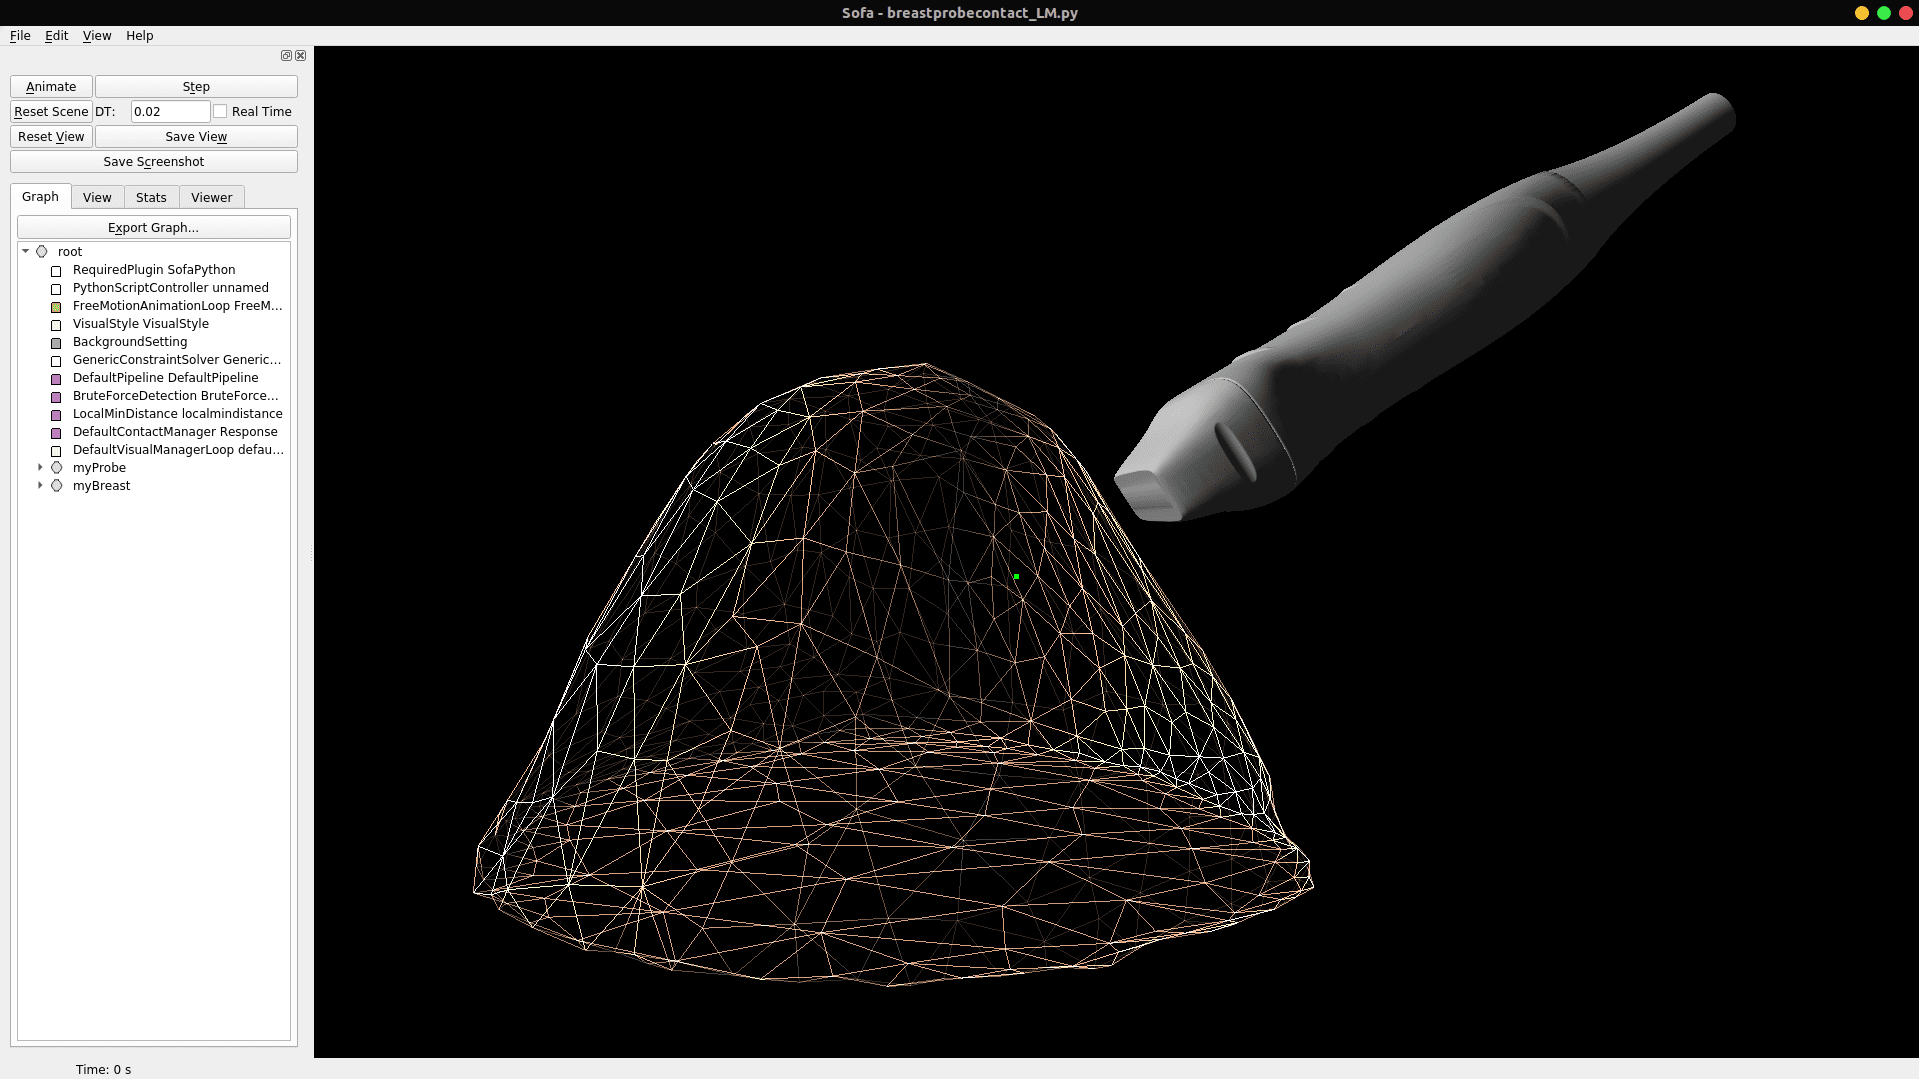
\includegraphics[width=0.49\textwidth]{images/future-work-sofa1.png}
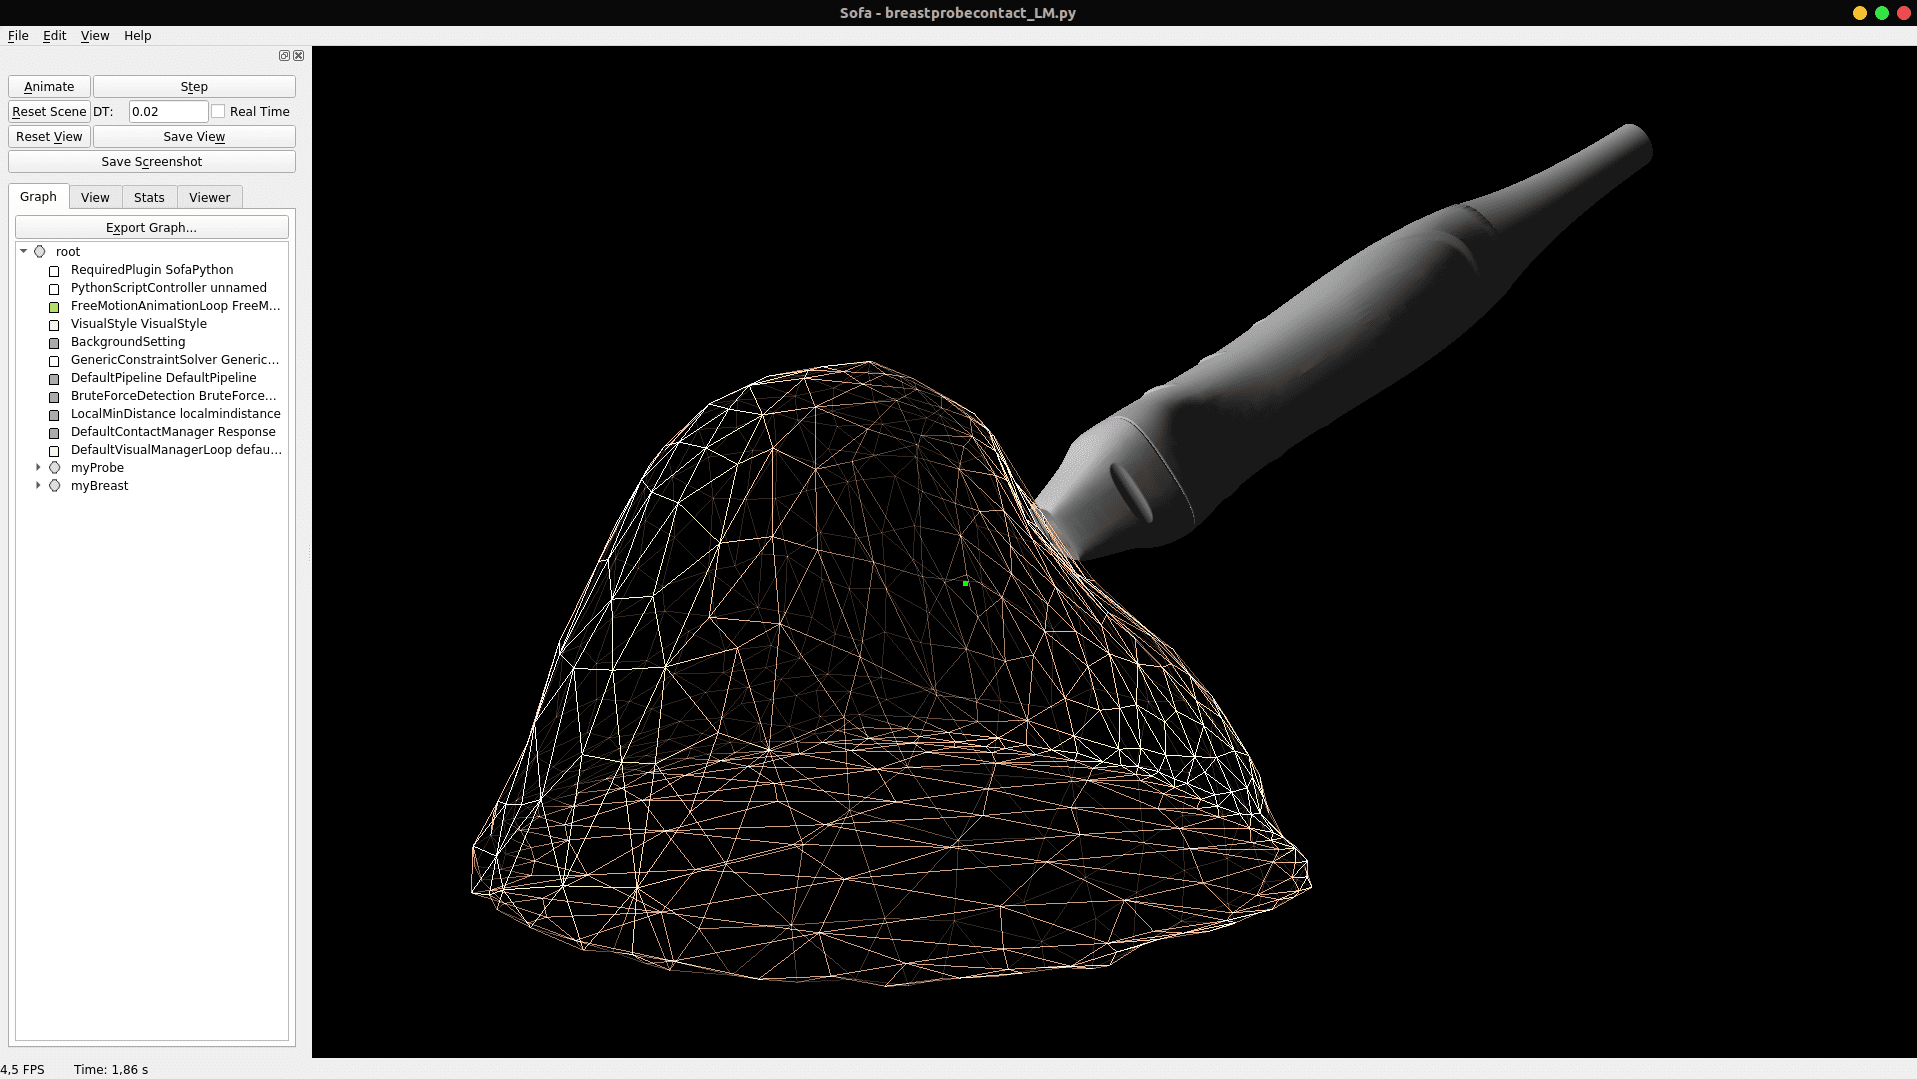
\includegraphics[width=0.49\textwidth]{images/future-work-sofa2.png}\\
\caption{Deformable tissue/organ medical simulation - Simulation of breast probing using the SOFA Framework. Screenshots from running the repository at
\url{https://gitlab.com/altairLab/probe-tissue-simulation}}
\end{figure}
\end{center}

\textbf{Advanced visualization and Haptics feedback} \\

\begin{center}
\begin{figure}[H]
\centering
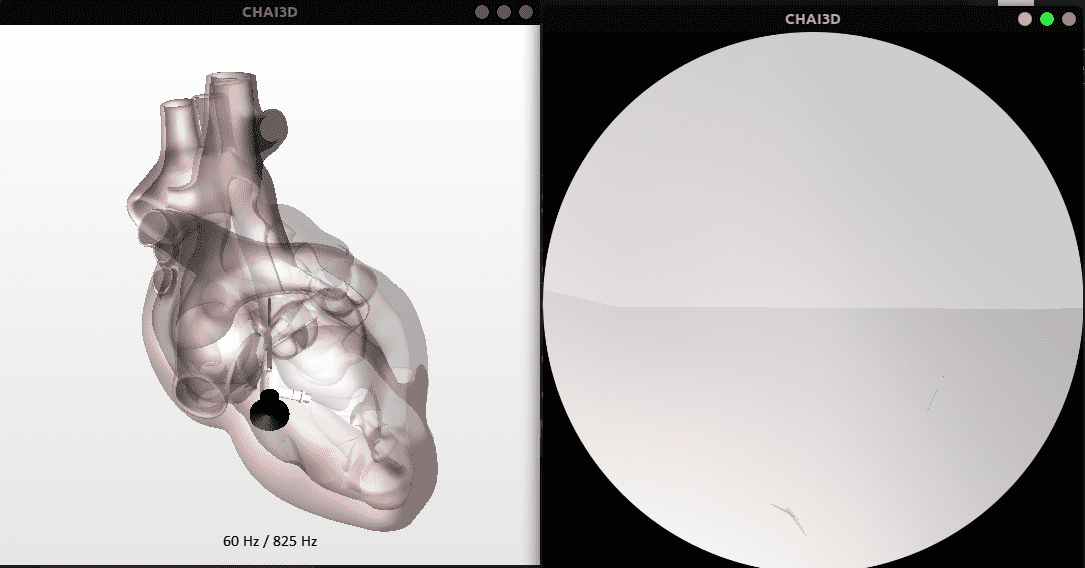
\includegraphics[width=0.7\textwidth]{images/future-work-chai3d.png}\\
\caption{Heart endoscopy medical simulation using the CHAI3D framework. Screenshots from running the repository at
\url{https://github.com/chai3d/chai3d}}
\end{figure}
\end{center}

\textbf{Applications of Machine Learning in Computer Vision and Path Planning} \\